\documentclass{compiladores}
\begin{document}

\begin{center}
{\LARGE Lista de Exercícios \#01}\\
{\bf Introdução à Compiladores e Análise Léxica}
\end{center}

\begin{listanumerada}
\item
Qual a diferença entre compilador e interpretador?

\item
Descreva todas as fases de um compilador. Por que existem duas fases de otimização?

\item
Qual a função do analisador léxico? Descreva o que é um \emph{token}, padrão e lexema.

\item
Qual o método mais eficiente de se detectar padrões na entrada de um analisador léxico?


\item
Descreva as {\bf linguagens} denotadas pelas seguintes expressões regulares:
\begin{lista}
  \item {\bf a(a|b)*a}
  \item {\bf (($\epsilon$|a)b*)*}
  \item {\bf (a|b)*a(a|b)(a|b)}
  \item {\bf a*ba*ba*ba*}
  \item {\bf (aa|bb)*((ab|ba)(aa|bb)*(ab|ba)(aa|bb)*)*}
\end{lista}

\item
Escreva as {\bf definições regulares} para cada uma das seguintes linguagens:
\begin{lista}
  \item Todas as cadeias de letra minúsculas que contêm as cinco vogais em ordem
  \item Todas as cadeias de dígitos com no máximo um dígito repetido
  \item Todas as cadeias de \emph{a}s e \emph{b}s que não contêm a subcadeia \emph{abb}
  \item Todos os números de ponto flutuante com sinal, fração e expoente \\
        (em geral, o sinal positivo é opcional: torne-o obrigatório)
  \item Todos os números hexadecimais (começando por \texttt{0x})
\end{lista}

\item
Faça {\bf diagramas de transição} para reconhecer as linguagens de
cada ER do exercício 5 e 6.

\item
Faça {\bf autômatos finitos} (deterministas ou não) para cada uma das linguagens do exercício 5.

\item
Crie uma {\bf tabela de transição} para cada um dos seguintes autômatos: \\
\begin{tabularx}{\textwidth}{XX}
\centering
a) 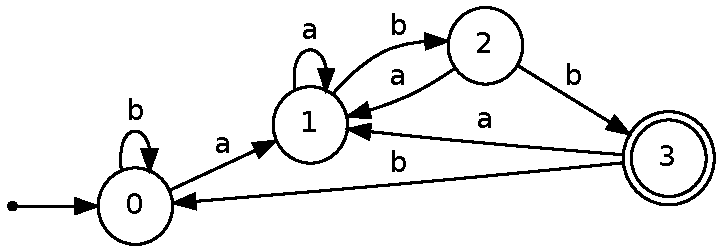
\includegraphics[width=.8\linewidth]{afd-1.pdf} &
b) 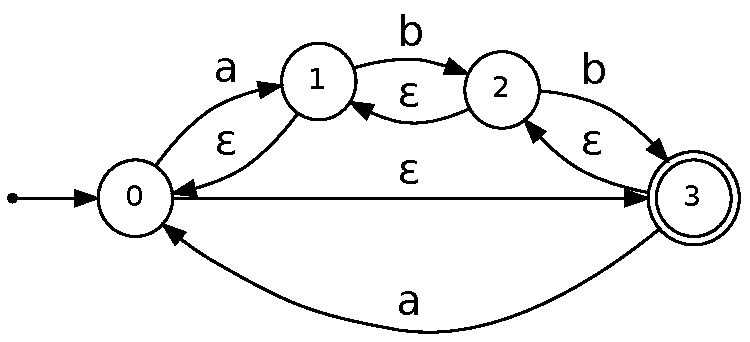
\includegraphics[width=.8\linewidth]{afnd-1.pdf}
\end{tabularx}
\begin{tabularx}{\textwidth}{X}
\centering
c) 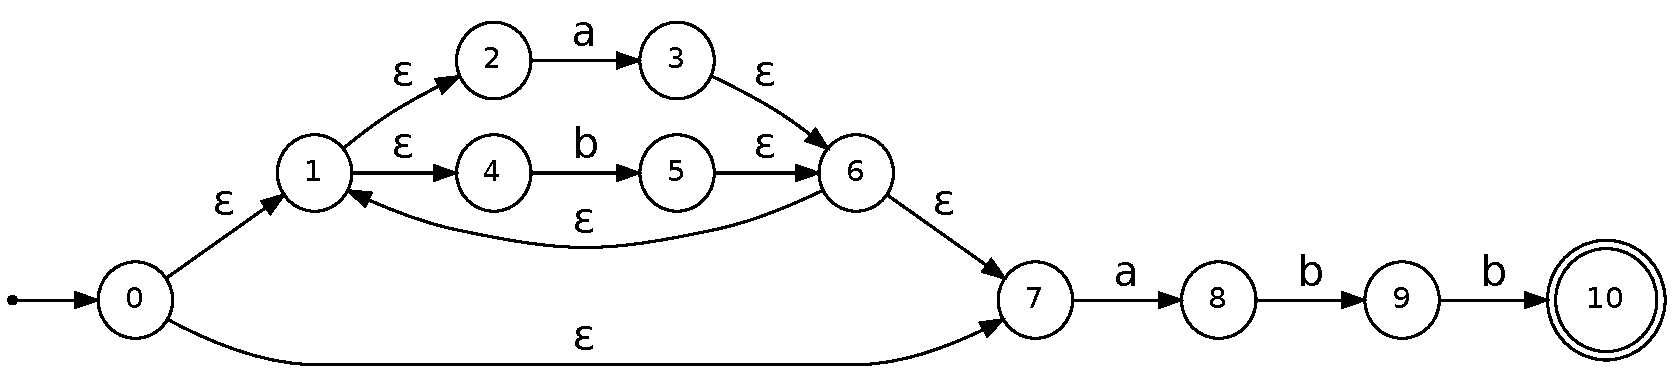
\includegraphics[width=.8\linewidth]{afnd_exemplo_3-34.pdf}
\end{tabularx}

\item
Converta os autômatos não deterministas do exercício 9 para
os determinitas correspondentes.

\item Converta as seguintes expressões regulares para autômatos
  finitos deterministas
\begin{lista}
  \item {\bf (a|b)*}
  \item {\bf (a*|b*)*}
  \item {\bf (($\epsilon$|b*)*}
  \item {\bf (a|b)*abb(a|b)*}
\end{lista}

\item
Transforme os diagramas de transição obtidos no exercício 7 para autômatos finitos determinitas.

\item
Por que um autômato finito determinista é a melhor forma de se implementar um analisador léxico?

\end{listanumerada}
\end{document}

